\section{Results}
\subsection{RQ1: How Does Representation Affect Relevant-Product Inclusion?}
Fact-equivalent orders repeatedly move judged-relevant products across operational cutoffs. Across three general encoders and two datasets, catalog-wide pair-micro VI@20 ranges from 4.42\% to 13.26\%; the product-specific encoder yields 6.07\% on WANDS and 7.22\% on ESCI. Figure~\ref{fig:crossmodel} reports query-macro estimates and uncertainty. These values describe crossing somewhere in a finite family of seven representations, rather than the expected loss from one arbitrary update.

\begin{figure}[t]
\centering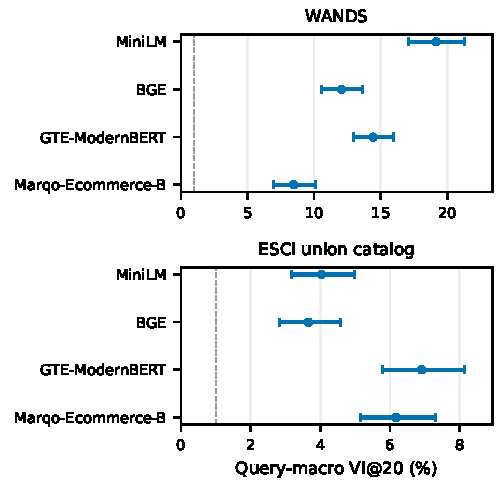
\includegraphics[width=\columnwidth]{figures/figure2_cross_model_vi.pdf}
\caption{Catalog-wide query-macro VI@20 with query-bootstrap 95\% CIs. The dashed 1\% line is a historical study threshold.}
\Description{Cross-model visibility instability on two product-search benchmarks with confidence intervals.}
\label{fig:crossmodel}
\end{figure}

The stricter target-only intervention fixes every competitor in C0 and replaces one relevant product at a time. WANDS pair-micro VI@20 is 12.72\%, 8.84\%, and 11.39\% for MiniLM, BGE, and GTE; ESCI values are 3.11\%, 3.16\%, and 6.68\%. Figure~\ref{fig:example} is drawn from this condition: only the target order changes between ranks 5 and 1,527. This supplies the controlled causal statement, while the catalog-wide experiment represents platform deployment where competitors change together.

The effect remains without encoder truncation. Among 8,536 WANDS Exact pairs whose seven complete inputs fit BGE, query-macro VI@20 is 8.69\% (CI [7.15,10.39]). Instability also omits stable failure: at Top-100, WANDS BGE has 8,384 highest-label pairs always included, 3,856 sometimes included, and 13,230 never included. ESCI has 3,995, 44, and 395, respectively. A method can therefore achieve zero VI by retrieving every relevant product or by omitting the same products consistently.

\subsection{RQ2: Do Visibility Rewriters Withstand Attribute Order?}
We next apply both frozen adapted E-GEO rewriters after each raw order. Figure~\ref{fig:optimization} separates mean target inclusion from order sensitivity on the fixed eight-query samples. With BGE on WANDS, Raw has 32.1\% mean inclusion@100 and 14.8\% VI. The heuristic has similar mean inclusion (32.3\%; paired change +0.25 points, CI [$-9.82$,14.42]) but more than doubles VI to 31.6\%. The technical prompt reaches 31.6\% mean inclusion and 23.2\% VI (change $-0.47$ points, [$-3.25$,2.19]). Thus neither rewriter improves the primary WANDS outcome, and both are more sensitive to order.

\begin{figure*}[t]
\centering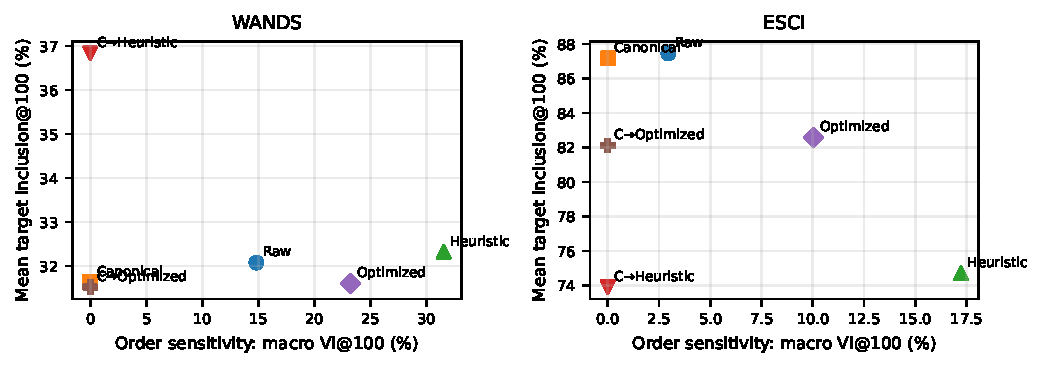
\includegraphics[width=.83\textwidth]{figures/optimization_quality_robustness.pdf}
\caption{Primary target-only BGE results at $K=100$. Each point reports query-macro mean inclusion and VI over seven input orders. Canonical-first inputs coincide across orders by construction and deterministic caching; zero VI therefore does not show that the generator itself is stable. Detailed values are in Appendix Table~\ref{tab:optimization}.}
\Description{Quality-versus-order-sensitivity plot for raw, canonical, and two adapted rewriting pipelines on WANDS and ESCI.}
\label{fig:optimization}
\end{figure*}

\begin{table*}[t]
\caption{Primary target-only BGE results at $K=100$. Mean inclusion, VI, and robust coverage (included under every tested order) are query-macro percentages; Never is pair-micro. This is a family of single-target counterfactual indexes, not one catalog Recall.}
\label{tab:optimization}\centering\small
\begin{tabular}{lrrrrrrrr}\toprule
&\multicolumn{4}{c}{WANDS}&\multicolumn{4}{c}{ESCI}\\
Method&Mean&VI&Robust&Never&Mean&VI&Robust&Never\\\midrule
Raw & 32.1 & 14.8 & 23.3 & 68.1 & 87.5 & 3.0 & 86.4 & 11.7\\
Canonical & 31.6 & 0.0 & 31.6 & 75.2 & 87.2 & 0.0 & 87.2 & 13.5\\
Heuristic & 32.3 & 31.6 & 19.0 & 48.7 & 74.7 & 17.2 & 66.0 & 18.0\\
C$\to$Heuristic & 36.8 & 0.0 & 36.8 & 70.0 & 73.9 & 0.0 & 73.9 & 27.0\\
Optimized & 31.6 & 23.2 & 20.2 & 69.4 & 82.6 & 10.0 & 77.1 & 13.5\\
C$\to$Optimized & 31.5 & 0.0 & 31.5 & 78.4 & 82.1 & 0.0 & 82.1 & 18.0\\
\bottomrule\end{tabular}
\end{table*}


On ESCI, Raw has 87.5\% mean inclusion and 3.0\% VI. The heuristic falls to 74.7\% and raises VI to 17.2\% (change $-12.74$ points, [$-23.49$,$-4.45$]); the technical prompt falls to 82.6\% with 10.0\% VI ($-4.89$ points, [$-9.43$,$-1.45$]). These are operational pipeline outcomes, not pure order effects, because most rewrites fail the fact check. Still, the deployment question is answered directly: an unguarded query-blind rewriter can amplify, rather than absorb, incoming representation variation.

Transition counts expose churn hidden by an average. Across 2,170 WANDS order--target trials at Top-100, the heuristic rescues 346 Raw misses but newly removes 176 Raw hits; on ESCI it rescues only 5 and newly removes 95 across 777 trials. The technical prompt rescues/removes 116/134 on WANDS and 1/36 on ESCI. Canonical-first heuristic outputs still replace 331/166 WANDS decisions and 0/106 ESCI decisions relative to Raw, even though their VI is zero. Counts are pair-micro events, whereas reported mean changes weight queries equally; their signs therefore need not coincide. The practical point is unchanged: net inclusion alone conceals which relevant products gain and lose access.

\begin{table*}[t]
\caption{Prespecified BGE contrasts in query-macro target inclusion@100 (percentage points; paired query-bootstrap 95\% CI). Holm-adjusted randomization results are in the artifact. Intervals crossing zero do not establish equivalence.}
\label{tab:optcontrasts}\centering\scriptsize
\begin{tabular}{lrrrrrr}\toprule
&$G_1-$Raw&$C\!\to\!G_1-G_1$&$C\!\to\!G_1-C$&$G_2-$Raw&$C\!\to\!G_2-G_2$&$C\!\to\!G_2-C$\\\midrule
WANDS & +0.2 [-9.8,+14.4] & +4.5 [-1.7,+12.5] & +5.2 [-4.0,+16.1] & -0.5 [-3.2,+2.2] & -0.1 [-2.9,+2.8] & -0.1 [-3.4,+4.0]\\
ESCI & -12.7 [-23.5,-4.5] & -0.8 [-4.8,+4.3] & -13.3 [-24.6,-4.1] & -4.9 [-9.4,-1.4] & -0.5 [-6.2,+4.4] & -5.1 [-10.6,-1.0]\\
\bottomrule\end{tabular}\end{table*}


Generation noise is a material alternative explanation. In the frozen eight-product stochastic control, WANDS same-input Top-100 crossing ranges from 16.7\% to 50.0\% across method/input cells, comparable to the within-replicate order VI of 16.7\%--50.0\%. ESCI has only two products per cell and is correspondingly uninformative. We therefore do not attribute the stochastic ranks solely to input order. The main experiment uses greedy decoding, but deterministic decoding is an implementation condition rather than a general stability guarantee.

\subsection{RQ3: Are Canonicalization and Factuality Guards Sufficient?}
Canonicalizing before generation makes all seven inputs identical. With deterministic content-addressed caching, $C\!\to\!G$ consequently has zero measured VI. It can nevertheless change inclusion. Relative to Canonical, the heuristic point estimate is +5.19 points on WANDS (CI [$-4.05$,16.13]) and $-13.27$ on ESCI ([$-24.60$,$-4.06$]); the technical prompt changes it by $-0.12$ ([$-3.37$,4.01]) and $-5.05$ points ([$-10.61$,$-0.96$]). Canonicalization controls incoming order; it does not ensure that the subsequent rewrite preserves facts or improves retrieval.

\begin{table}[t]\caption{Adapted-generator factuality and local cost. Strict pass uses the frozen rule checker; Exec. and Guard are fallback rates. Minutes are unique cached batched GPU generation time; monetary API cost is zero.}\label{tab:optfacts}\centering\scriptsize
\begin{tabular}{llrrrrrr}\toprule Data&Method&$n$&Pass\%&Exec.\%&Guard\%&Tok.&min\\\midrule
WANDS & G1 & 2170 & 0.0 & 17.9 & 100.0 & 366 & 171.7\\
WANDS & CG1 & 310 & 0.0 & 14.5 & 100.0 & 400 & 25.1\\
WANDS & G2 & 2170 & 0.0 & 72.7 & 100.0 & 501 & 315.6\\
WANDS & CG2 & 310 & 0.0 & 80.3 & 100.0 & 508 & 44.6\\
ESCI & G1 & 777 & 7.6 & 12.9 & 92.4 & 324 & 19.3\\
ESCI & CG1 & 111 & 8.1 & 9.9 & 91.9 & 330 & 1.3\\
ESCI & G2 & 777 & 0.0 & 67.2 & 100.0 & 504 & 27.7\\
ESCI & CG2 & 111 & 0.0 & 65.8 & 100.0 & 505 & 1.8\\
\bottomrule\end{tabular}\end{table}


Table~\ref{tab:optfacts} explains why the favorable WANDS heuristic point estimate is not credible evidence of fact-preserving optimization. No WANDS output passes the conservative field-level checker. On ESCI, only 7.6\% of raw-order and 8.1\% of canonical-input heuristic outputs pass; no technical-prompt output passes. The technical prompt reaches the 512-token output cap for 65.8\%--80.3\% of cells, while the heuristic truncates 9.9\%--17.9\%. WANDS source records also contain conflicting fields that a valid rewrite must retain rather than silently reconcile. The checker is deliberately strict and is not human ground truth, but the common-valid support is only two ESCI products for the heuristic and empty elsewhere, far too small for an effectiveness claim.

The component audit shows that failure is not only truncation. For WANDS raw-order heuristic outputs, 99.7\% omit at least one checked attribute value, 98.8\% omit a source number, 70.7\% omit a source color, and 21.1\% introduce a new number; 83.2\% of evaluated rows originate from products containing a source-field conflict. ESCI has no such conflict flag, yet its heuristic omits a checked attribute in 84.9\% and a number in 75.7\%, while adding a number in 18.3\%. The technical prompt adds numbers in 62.6\% of WANDS and 65.9\% of ESCI raw-order outputs. These rules deliberately count any missing constrained value, so they should be read as error flags rather than calibrated semantic-quality probabilities.

The prespecified guard returns raw canonical text for truncation, empty output, or any fact-check failure. Consequently, every guarded WANDS and technical-prompt cell equals Canonical. For ESCI heuristic+BGE, guarded mean inclusion@100 is 86.2\% versus 87.2\% for Canonical and VI is zero; with MiniLM it is 75.3\% versus 75.6\% and VI is 1.0\%. The residual MiniLM sensitivity comes from the few order-specific outputs that pass. The guard prevents unsupported text from reaching retrieval, but supplies no improvement over canonical preprocessing.

Full-catalog canonical results provide the deployable comparison that target interventions cannot. Recall@100 changes by +0.07 points on WANDS+BGE, +0.07 on ESCI+BGE, and +0.28 on ESCI+MiniLM, with all three intervals spanning zero. WANDS+MiniLM falls by 1.83 points (CI [$-3.17$,$-0.64$]). Canonical sorting is therefore a simple structural defense, but its relevance cost is encoder-dependent and intervals containing zero do not prove equivalence.

\subsection{RQ4: What Transfers, and What Does Robustness Cost?}
The generated text transfers without regeneration to MiniLM, but the direction does not stabilize. On WANDS, the heuristic changes inclusion@100 by $-3.77$ points relative to Raw (CI [$-14.36$,6.28]); the technical prompt changes it by +1.62 ([$-2.68$,6.37]). On ESCI, corresponding changes are +0.72 ([$-3.78$,5.72]) and $-0.89$ points ([$-4.30$,2.49]). No cell supports a consistent cross-encoder gain. The earlier development-selected appearance-first rule similarly loses 1.75 points on WANDS MiniLM ([$-3.00$,$-0.63$]), reinforcing that representation choices do not transfer automatically.

The local generator incurred no API charge, but the frozen primary outputs required about 10.1 GPU-hours of measured generation, plus 1.4 hours for the stochastic control. The technical prompt accounts for most compute because its outputs approach the cap. This exceeded the planned eight-hour generation stop; the deviation is disclosed because completion was not selected by observed ranks and no sample, prompt, or outcome was changed. In contrast, raw canonical sorting needs no language-model inference.

Platform-side alternatives retain different tradeoffs. Equal-weight hybrid retrieval improves Recall@100 from 0.632 to 0.681 on WANDS and from 0.910 to 0.915 on ESCI. A four-view centroid raises WANDS recall by 1.22 points (CI [0.34,2.29]) but is not monotonically improved by seven views. The invariant set-mean representation has small, statistically inconclusive historical cNDCG changes, yet lowers new-query ESCI Recall@100 by 2.03 points ([$-3.15$,$-0.90$]). Finally, fixed-text reranking changes WANDS final Recall@20 by +0.66 points at a 100-candidate budget ([$-0.03$,1.58]); expanding Original from 100 to 500 candidates yields +1.13 ([$0.08$,2.41]). Reranking can reorder candidates, but it cannot recover products it never receives.
